
%----------------------------------------------------------------------------------------
%	PACKAGES AND OTHER DOCUMENT CONFIGURATIONS
%----------------------------------------------------------------------------------------

\documentclass[12pt]{article} % Default font size is 12pt, it can be changed here

\usepackage{geometry} % Required to change the page size to A4
\geometry{a4paper} % Set the page size to be A4 as opposed to the default US Letter

\usepackage{graphicx} % Required for including pictures

\usepackage{float} % Allows putting an [H] in \begin{figure} to specify the exact location of the figure
%\usepackage{wrapfig} % Allows in-line images such as the example fish picture

%\usepackage{lipsum} % Used for inserting dummy 'Lorem ipsum' text into the template

%\linespread{1.2} % Line spacing

%\setlength\parindent{0pt} % Uncomment to remove all indentation from paragraphs


\begin{document}

%----------------------------------------------------------------------------------------
%	TITLE PAGE
%----------------------------------------------------------------------------------------

\begin{titlepage}

\newcommand{\HRule}{\rule{\linewidth}{0.5mm}} % Defines a new command for the horizontal lines, change thickness here

\center % Center everything on the page

\textsc{\LARGE La Sapienza}\\[1.5cm] % Name of your university/college
\textsc{\Large Fundamentals of Computer Graphics}\\[0.5cm] % Major heading such as course name

\HRule \\[0.4cm]
{ \huge \bfseries Homework 4}\\[0.4cm] % Title of your document
\HRule \\[1.5cm]

\begin{minipage}{0.4\textwidth}
\begin{flushleft} \large
\emph{Author:}\\
Sara \textsc{Di Bartolomeo} % Your name
\end{flushleft}
\end{minipage}
~
\begin{minipage}{0.4\textwidth}
\begin{flushright} \large
\emph{} \\
 \textsc{} % Supervisor's Name
\end{flushright}
\end{minipage}\\[4cm]

{\large \today}\\[3cm] % Date, change the \today to a set date if you want to be precise

%\includegraphics{Logo}\\[1cm] % Include a department/university logo - this will require the graphicx package

\vfill % Fill the rest of the page with whitespace

\end{titlepage}


%----------------------------------------------------------------------------------------
%	INTRODUCTION
%----------------------------------------------------------------------------------------

\section{Tests} % Major section

%------------------------------------------------

\subsection{Textures} % Sub-section

The first test shows an example of how textures can be applied to a plane mesh.\\
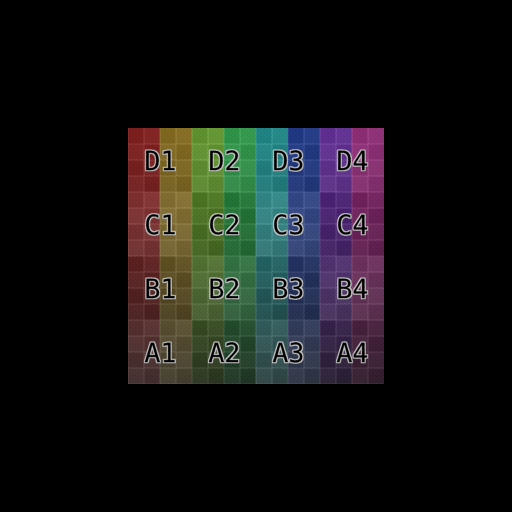
\includegraphics[width=\linewidth]{Homework4/tests/01_textured.png}
Time: 00:00:01,01

%------------------------------------------------

\subsection{Area Light} % Sub-section

This test shows the effect of an area light (that is positioned behind the camera) on two meshes.\\
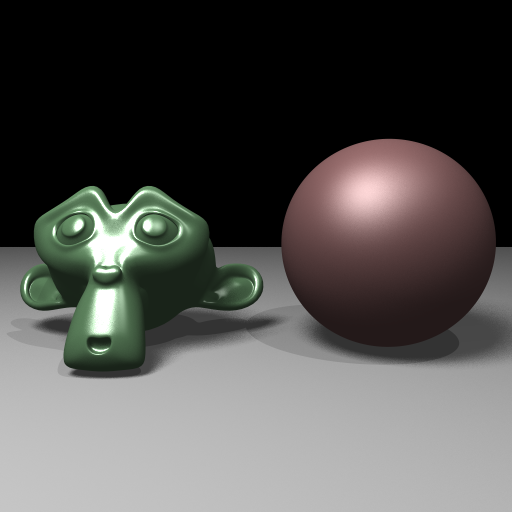
\includegraphics[width=\linewidth]{Homework4/tests/02_area.png}
Time: 00:00:35,44

%------------------------------------------------

\subsection{Environment Light} 

This test shows the effect of environment light on the same two meshes as before. As opposed to the example before this, here the light we see on the meshes comes from the skybox, assuming the same color as the texture used.\\
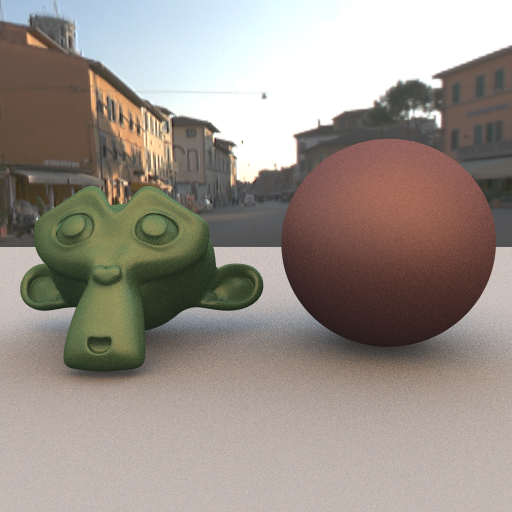
\includegraphics[width=\linewidth]{Homework4/tests/03_env_correct.png}
Time: 00:00:35,97
\\\\
This second image shows the effect of environment light with a different texture.
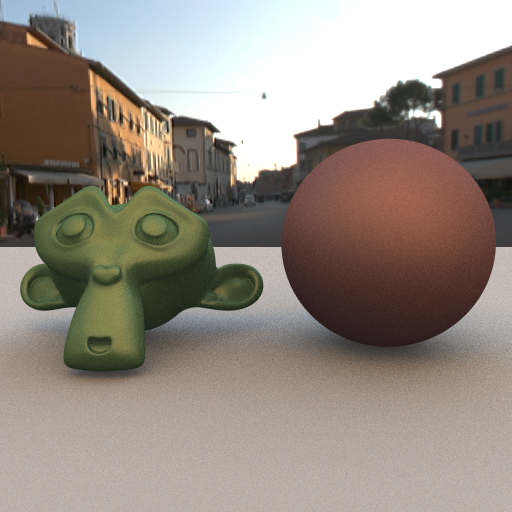
\includegraphics[width=\linewidth]{Homework4/tests/03_env.png}


\subsection{Light} 

This test shows how light emitted from two planes (one of which is textured) affects the surface of a sphere. The effect of area light can be clearly seen.\\
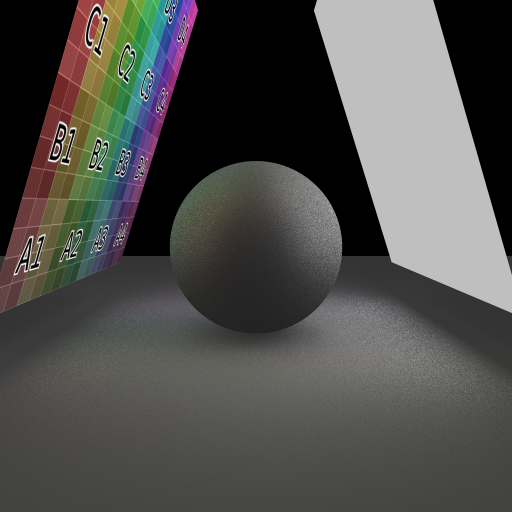
\includegraphics[width=\linewidth]{Homework4/tests/04_light.png}
Time: 00:00:14,97

\subsection{Materials} 

In this test, we show the effect of microfacet on a material. Microfaceting a material means assuming that the surface of said material isn't perfectly smooth, but is composed of many small facets, thus producing a slightly blurred reflection as opposed to a perfectly sharp reflected image.\\
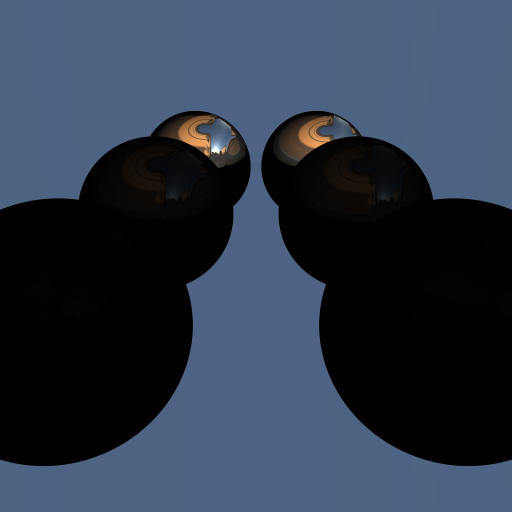
\includegraphics[width=\linewidth]{Homework4/tests/05_materials.png}
Time: 00:01:17,77

\subsection{Direct Light} 

Another example of the effect of area light is shown here. Smooth shadows that are obtained with area lights are clearly visible.\\
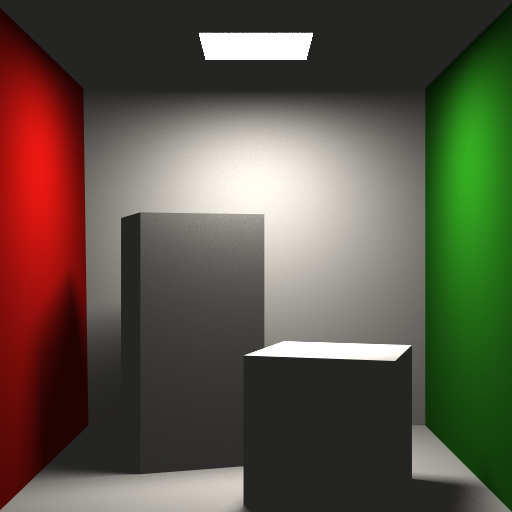
\includegraphics[width=\linewidth]{Homework4/tests/06_cb_direct.png}
Time: 00:02:34,54


\subsection{Indirect Light} 

Here we can see the effect of indirect light. The difference with the example before this is that here we also consider the fact that surfaces not only absorb but also reflect a part of the light that hits them.\\
In the image, a red light comes from the left and a green one from the light, but there are no added lights from the example before. This is just the effect of reflected lights on the two colored walls.\\
The effect is obtained by recursively calculating the pathtrace result, each time recalculating the ray direction and origin.\\
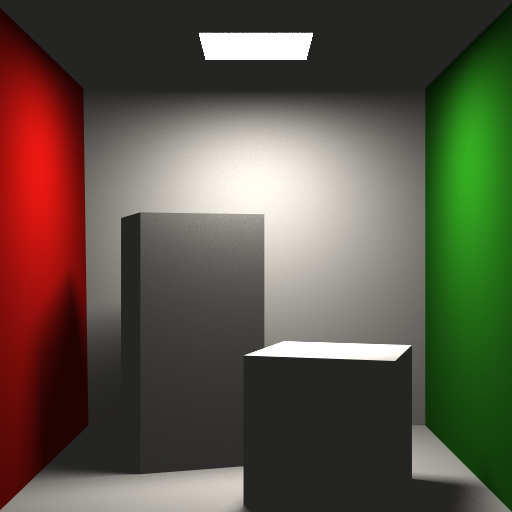
\includegraphics[width=\linewidth]{Homework4/tests/07_cb_indirect.png}
Time: 00:07:28,99

\subsection{Custom}
This last one shows many of the features of the tests before in a single image. The macbook is composed by different materials, each one with its own properties:
\begin{list}{-}{spacing}
	\item The body is made of a microfaceted, specular material.
	\item The keyboard instead needed to be dull, therefore is not specular at all, and has a texture with the key symbols.
	\item The screen is emissive and has an emissive texture, so it emits a colored light.
	\item Other small components are dull as well.
\end{list}
The image also features indirect light and an area light positioned behind the camera.\\\\
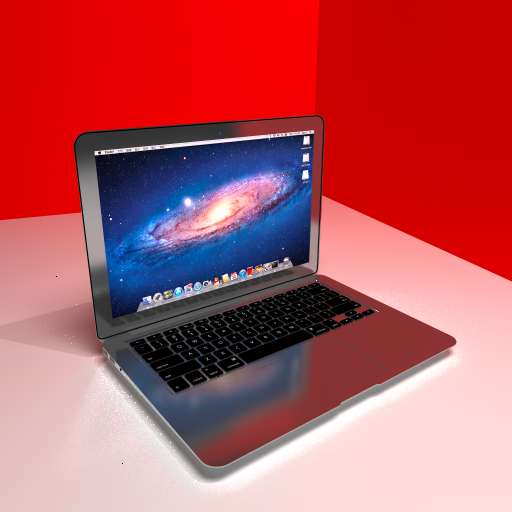
\includegraphics[width=\linewidth]{Homework4/tests/macbook.png}
Time: 00:53:22,03 


%	MAJOR SECTION X - TEMPLATE - UNCOMMENT AND FILL IN
%----------------------------------------------------------------------------------------

%\section{Content Section}

%\subsection{Subsection 1} % Sub-section

% Content

%------------------------------------------------

%\subsection{Subsection 2} % Sub-section

% Content

%----------------------------------------------------------------------------------------
%	CONCLUSION
%----------------------------------------------------------------------------------------



%\lipsum[12-13]


%----------------------------------------------------------------------------------------

\end{document}